\documentclass[11pt]{article}
\usepackage[margin=0.72in]{geometry}
\usepackage{amsmath,booktabs,graphicx,microtype}
\usepackage{tikz}
\usepackage{pgfplots}
\pgfplotsset{compat=1.18}
\usepackage[hidelinks]{hyperref}
\setlength{\columnsep}{0.25in}
\setlength{\parindent}{0pt}
\setlength{\parskip}{3pt}
\title{Estimating $\pi$ with OpenMP report}
\author{Pria Wisetmongkolchai\\CS 431/531 --- Parallel Programming}
\begin{document}
\maketitle
\section{Methods}
\textbf{Numerical integration.} The upper semicircle has area $\pi/2$
\begin{equation}
\pi = 2\int_{-1}^{1}\sqrt{1-x^2}\,dx.
\label{eq:integral}
\end{equation}


\textbf{Monte Carlo.} Generate $N=10^6$ points $(x,y)$ in the unit square. A point is a hit if $x^2+y^2\leq1$; then
\begin{equation}
\widehat\pi=4\frac{N_{\mathrm{hits}}}{N}.
\end{equation}
\section{Experimental Setup}
 $p\in\{1,2,4,8\}$ threads. Each configuration was run 20 times at $N=10^6$. Table~\ref{tab:results} gives mean elapsed times. The serial baseline was remeasured at each thread setting. 

\begin{table}[t]
\centering
\caption{Mean elapsed time over 20 runs (milliseconds).}
\label{tab:results}
\small
\begin{tabular}{@{}rrrrr@{}}
\toprule
Threads & Serial & Atomic int. & Monte Carlo & MC $S_p$ \\
\midrule
1 & 2.233 & 11.778 & 10.193 & 1.00 \\
2 & 2.242 & 45.934 & 5.294 & 1.93 \\
4 & 2.265 & 53.890 & 2.794 & 3.65 \\
8 & 2.260 & 57.428 & 1.418 & 7.19 \\
\bottomrule
\end{tabular}
\end{table}

\begin{figure}[t]
\centering
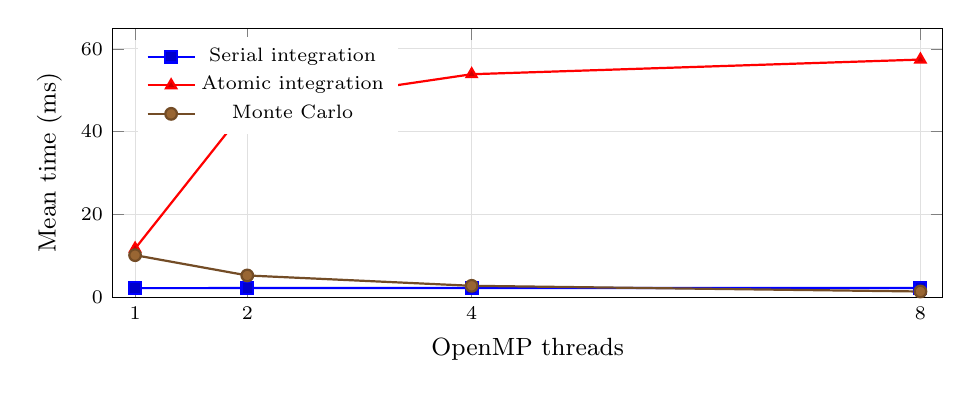
\begin{tikzpicture}
\begin{axis}[
width=\columnwidth,height=5.0cm,
 xlabel={OpenMP threads},ylabel={Mean time (ms)},
 xtick={1,2,4,8},xmin=0.8,xmax=8.2,
 ymin=0,ymax=65,
 grid=major,grid style={black!12},
 legend style={font=\scriptsize,at={(0.03,0.97)},anchor=north west,fill=white,draw=none},
 tick label style={font=\scriptsize},label style={font=\small},
 mark size=2.1pt]
\addplot+[thick,mark=square*] coordinates {(1,2.233)(2,2.242)(4,2.265)(8,2.260)};
\addlegendentry{Serial integration}
\addplot+[thick,mark=triangle*] coordinates {(1,11.778)(2,45.934)(4,53.890)(8,57.428)};
\addlegendentry{Atomic integration}
\addplot+[thick,mark=*] coordinates {(1,10.193)(2,5.294)(4,2.794)(8,1.418)};
\addlegendentry{Monte Carlo}
\end{axis}
\end{tikzpicture}
\caption{Measured runtime as thread count increases. Atomic integration becomes slower; Monte Carlo becomes faster.}
\label{fig:time}
\end{figure}

\begin{figure}[t]
\centering
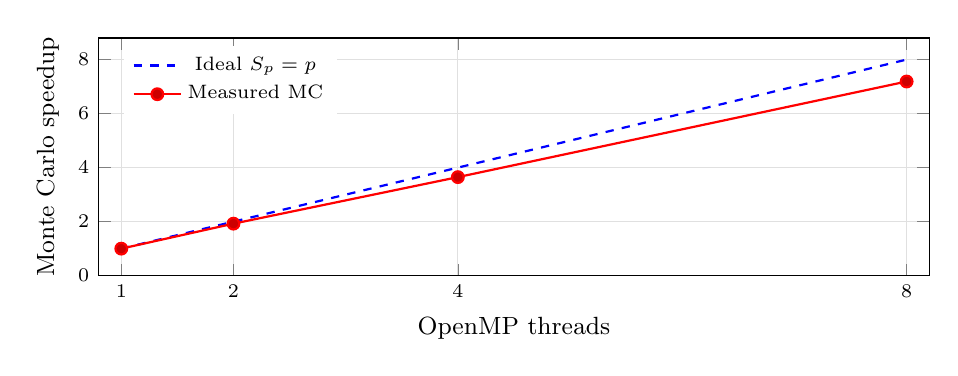
\begin{tikzpicture}
\begin{axis}[
width=\columnwidth,height=4.6cm,
 xlabel={OpenMP threads},ylabel={Monte Carlo speedup},
 xtick={1,2,4,8},xmin=0.8,xmax=8.2,
 ymin=0,ymax=8.8,grid=major,grid style={black!12},
 legend style={font=\scriptsize,at={(0.03,0.97)},anchor=north west,fill=white,draw=none},
 tick label style={font=\scriptsize},label style={font=\small},
 mark size=2.1pt]
\addplot+[thick,dashed,mark=none] coordinates {(1,1)(2,2)(4,4)(8,8)};
\addlegendentry{Ideal $S_p=p$}
\addplot+[thick,mark=*] coordinates {(1,1)(2,1.9254)(4,3.6482)(8,7.1883)};
\addlegendentry{Measured MC}
\end{axis}
\end{tikzpicture}
\caption{Monte Carlo speedup $S_p=T_1/T_p$, using its one-thread time as baseline.}
\label{fig:speedup}
\end{figure}

\section{Findings and Discussion}
\textbf{1. Serial integration.} The serial program reported $\widehat\pi=3.1415926503$ at each thread setting. Its mean runtimes for the nominal settings of 1, 2, 4, and 8 threads were 2.233, 2.242, 2.265, and 2.260 ms, respectively. These times differ by 0.032 ms across the four settings (Table~\ref{tab:results}). This is expected, the serial implementation performs the work sequentially and does not use additional OpenMP threads even when the job requests a higher thread count.

\textbf{2. Parallel integration.} The atomic shared-sum implementation reported $\widehat\pi=3.1415926503$ at all four thread counts, but adding threads did not improve its runtime. The averages rose from 11.778 ms (1 thread) to 45.934 ms (2 threads), 53.890 ms (4 threads), and 57.428 ms (8 threads). Figure~\ref{fig:time} shows the upward trend. Although iterations are distributed among threads, an atomic update to the same shared sum occurs repeatedly, outweighing the benefit of parallel loop iterations. The eight-thread run was about 4.88 times slower than the one-thread atomic run.

\textbf{3. Monte Carlo.} Unlike numerical integration, Monte Carlo uses random points; the reported estimates were 3.1424480000, 3.1393560000, 3.1408240000, and 3.1418960000 for 1, 2, 4, and 8 threads, respectively. Its mean runtimes decreased from 10.193 ms (1 thread) to 5.294 ms (2 threads), 2.794 ms (4 threads), and 1.418 ms (8 threads). As Fig.~\ref{fig:speedup} shows, these correspond to speedups of 1.93$\times$, 3.65$\times$, and 7.19$\times$ relative to one thread; the eight-thread efficiency is approximately 89.9\%. Independent random-point tests can be distributed with little synchronization compared with an atomic update on every integration iteration. The four estimates do not become progressively more accurate with thread count.

\textbf{4. Critical section versus atomic.} Both OpenMP \texttt{critical} and \texttt{atomic} protect concurrent access to a shared variable. A \texttt{critical} region permits an arbitrary block of code but allows only one thread at a time to execute that protected region. \texttt{atomic} protects a supported memory update, such as adding one iteration's contribution to the shared sum, and is generally a narrower operation. In one separate test, the \texttt{critical} implementation took 75.388 ms while \texttt{atomic} took 58.658 ms; both returned $3.1415926503$. In that test, \texttt{atomic} was approximately 22.2\% faster, but these are individual measurements, not 20-run averages. Both designs still require synchronization on every iteration, so neither avoids the central shared-sum bottleneck. An OpenMP \texttt{reduction} using private partial sums would be a useful follow-up experiment, not a measured result in this report.

\section{Conclusion}
The results show that the number of threads alone does not determine speed. Serial integration remained stable near 2.25 ms regardless of the requested thread count. Atomic parallel integration became slower as synchronization contention increased, despite producing the same $\pi$ estimate. By contrast, Monte Carlo benefited from independent work and achieved 7.19$\times$ speedup at eight threads, though its estimated $\pi$ varied between runs. The separate \texttt{critical}/\texttt{atomic} comparison also suggests that synchronization method affects runtime, and motivates testing thread-local reduction in future work.
\end{document}